\documentclass{standalone}
\usepackage{tikz}
\usepackage{newtxmath}
\usetikzlibrary{decorations.markings,decorations.pathmorphing,arrows,positioning,automata,calc,patterns}

\colorlet{myred}{red!70!black}
\colorlet{mygreen}{green!60!black}

\begin{document}

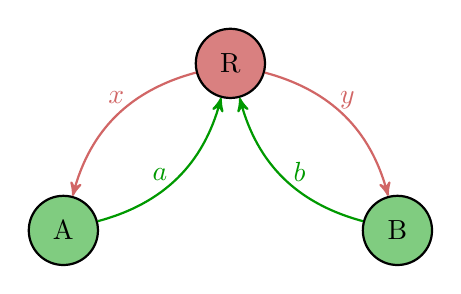
\begin{tikzpicture}[->, >=stealth', auto, semithick, node distance=3cm]
    \tikzstyle{every state}=[draw=black,thick,text=black,scale=1]

    \node[state,fill=myred!50]    (R)                     {R};
    \node[state,fill=mygreen!50]   (A)[below left of=R]    {A};
    \node[state,fill=mygreen!50]   (B)[below right of=R]   {B};

    \path
    (R) edge[bend right,above,myred!60,thick]	node[yshift=1pt]{$x$}	(A)
    (R) edge[bend left,above,myred!60,thick]	node[yshift=-1pt,xshift=1pt]{$y$}	(B)
    (A) edge[bend right,left,mygreen,thick]	node[yshift=1pt]{$a$}	(R)
    (B) edge[bend left,right,mygreen,thick]	node[yshift=2pt]{$b$}	(R);

\end{tikzpicture}

\end{document}